\documentclass[a4paper,11pt,UTF8]{article}
\usepackage{ctex}
\usepackage{amsmath,amsthm,amssymb,amsfonts}
\usepackage{amsmath}
\usepackage[a4paper]{geometry}
\usepackage{graphicx}
\usepackage{microtype}
\usepackage{siunitx}
\usepackage{booktabs}
\usepackage[colorlinks=false, pdfborder={0 0 0}]{hyperref}
\usepackage{cleveref}
\usepackage{esint} 
\usepackage{graphicx}
\usepackage{ragged2e}
\usepackage{pifont}
\usepackage{extarrows}
\usepackage{mathptmx}
\usepackage{float}
\usepackage{caption}
\captionsetup[figure]{name={Figure}}

\title{Microelectronics Circuit Analysis and Design Homework(9th)}
\author{Yuejin Xie \quad U202210333}
\date{Oct 14th, 2023}
\begin{document}
\maketitle
7.3 Consider the circuit in Figure P7.3. (a) Derive the expression for the voltage transfer function $T(s) = V_o(s)/V_i (s)$.(b) What is the time constant associated with this circuit? (c) Find the corner frequency. (d) Sketch the Bode magnitude plot of the voltage transfer function.
\begin{figure}[H]
	\centering
	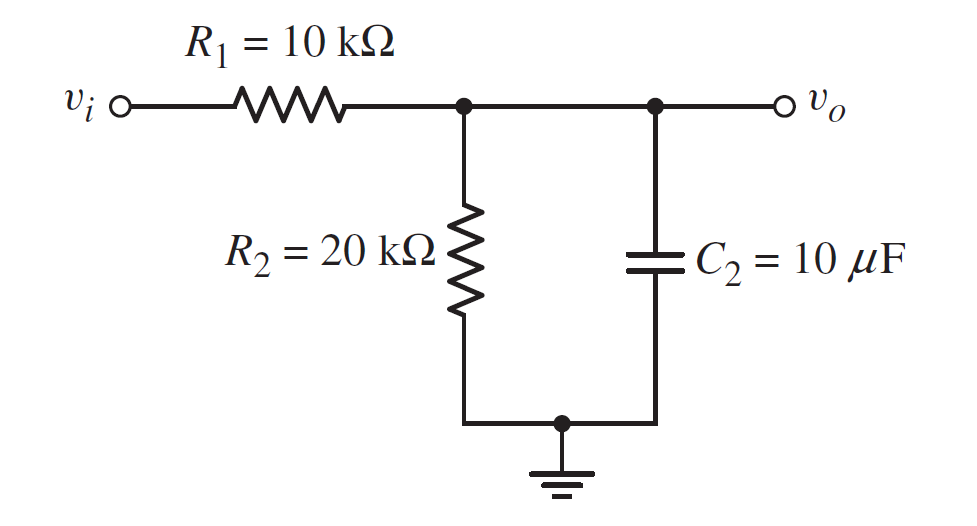
\includegraphics[scale=0.3]{MD7.3}
	\caption{Problem 7.3}
\end{figure}
7.12 For the circuit shown in Figure P7.12, the parameters are $R_1 = 10 \mathrm{k\Omega},
R_2 = 10 \mathrm{k\Omega}, R_3 = 40 \mathrm{k\Omega}$, and $C = 10\mathrm{\mu F}$. (a) What is the value of the voltage
transfer function $V_o/V_i$ at very low frequencies? (b) Determine the value of the voltage transfer function at very high frequencies. (c) Derive the expression for the voltage transfer function $T (s) = V_o(s)/V_i(s)$. Put the expression in the form$ T(s) = K(1 + s\tau_A)/(1 + s\tau_B)$. What are the values
of $K, \tau_A,$ and $\tau_B$.
\begin{figure}[H]
	\centering
	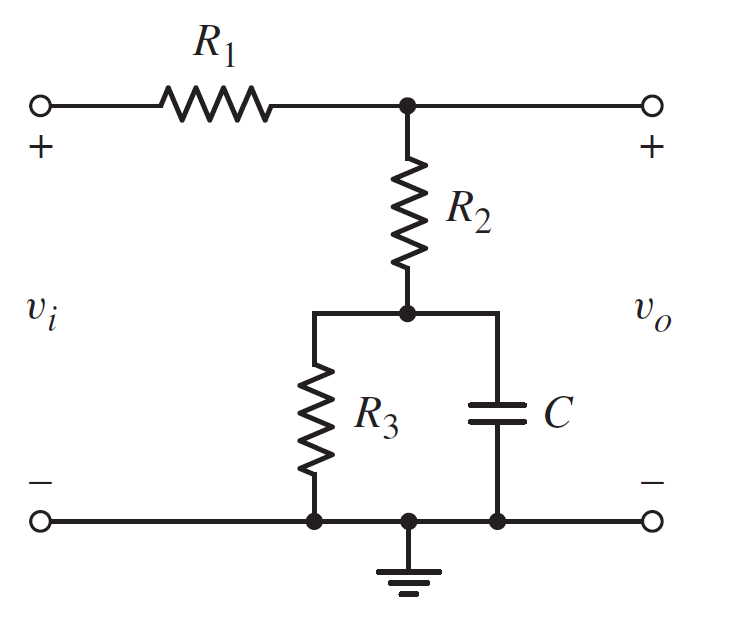
\includegraphics[scale=0.3]{MD7.12}
	\caption{Problem 7.12}
\end{figure}
7.17 For the common-emitter circuit in Figure P7.17, the transistor parameters are: $\beta = 100, V_{BE(on)} = 0.7 $V, and $V_A =\infty$. (a) Calculate the lower corner frequency. (b) Determine the midband voltage gain. (c) Sketch the Bode plot of the voltage gain magnitude.
\begin{figure}[H]
	\centering
	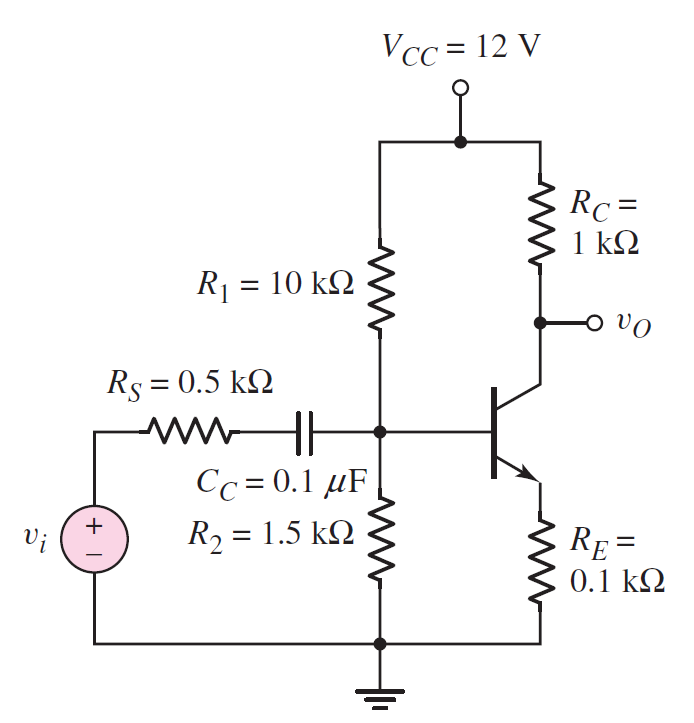
\includegraphics[scale=0.3]{MD7.17}
	\caption{Problem 7.17}
\end{figure}
7.26 The parameters of the transistor in the circuit in Figure P7.26 are $K_p =1 \mathrm{mA/V^2}, V_{TP} = -1.5\mathrm{V},$ and $\lambda=0$. (a) Determine the quiescent and small-signal parameters of the transistor. (b) Find the time constants associated with $C_{C1}$ and $C_{C2}$. (c) Is there a dominant pole frequency? Estimate the -3 dB frequency.
\begin{figure}[H]
	\centering
	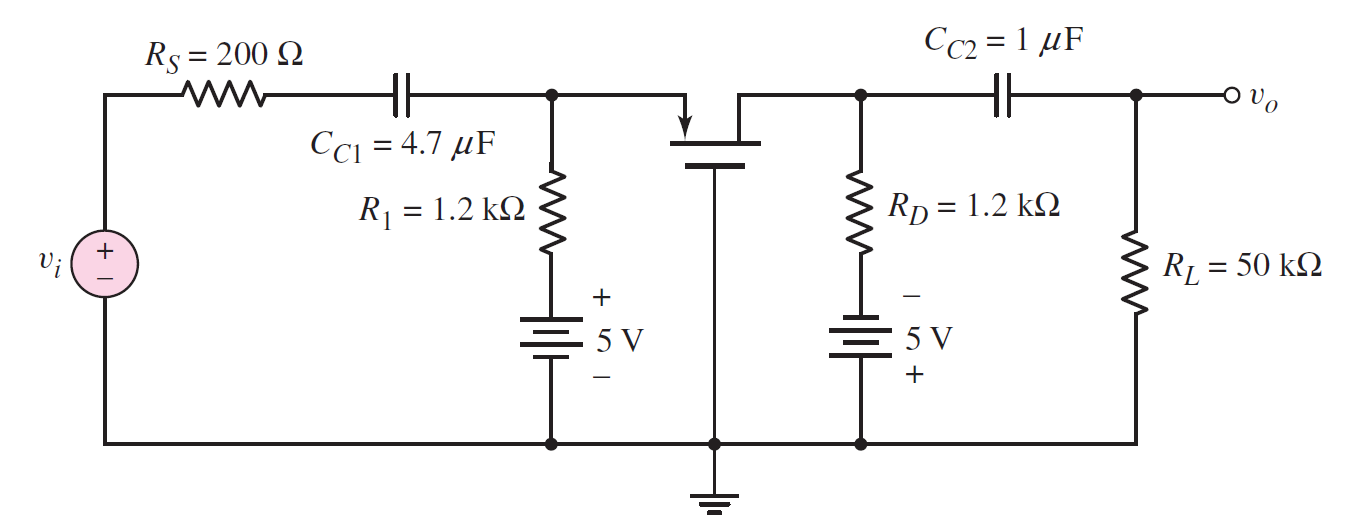
\includegraphics[scale=0.3]{MD7.26}
	\caption{Problem 7.26}
\end{figure}
\end{document}